%   MSc Business Analytics Dissertation
%   Format based on skeleton template provided as part of module MIS40750
%
%   Title:     Optimising the design of buffer preparation in bioprocessing
%              facilities
%   Author:    Sean Tully
%
%   Chapter 5: Results
%
%   Change Control:
%   When     Who   Ver  What
%   -------  ----  ---  --------------------------------------------------------
%   06Jun16  ST    0.1  Begun 
%

\chapter{Results}\label{C.results}

\begin{quote}
Bosh! Stephen said rudely.
A man of genius makes no mistakes.
His errors are volitional and are the portals of discovery.

\hspace{2cm}--- James Joyce, \emph{Ulysses}
\end{quote}

\section{Output Data}\label{S.outputdata}

This section describes the format of the outputs generated by the model, rather
than the values of the results themselves, which are discussed in detail in 
\hyperref[C.results]{Chapter \ref*{C.results}}.

The primary aim is to generate a list of the required preparation volumes.
For the random example used in this chapter, solution of the model yields
the results in \hyperref[tbl.reqvessels]{Table \ref*{tbl.reqvessels}}.

\begin{table}[h!]
    \centering
    \caption{Required preparation vessels for random example}
    \label{tbl.reqvessels}
    \begin{tabular}{r}
        vessel size\\ \hline
        \SI{2000}{\litre}\\
        \SI{8000}{\litre}\\
        \SI{25000}{\litre}\\
        \SI{30000}{\litre}\\
    \end{tabular}
\end{table}

While \hyperref[tbl.reqvessels]{Table \ref*{tbl.reqvessels}} gives the
essential information allowing the buffer preparation area to be sized and
costed, it may be more instructive to return a matrix showing where each buffer
is to be prepared. 
\hyperref[tbl.bvmatrix]{Table \ref*{tbl.bvmatrix}} shows \emph{one possible}
vessel assignment for the random example.

\begin{table}[t]
    \centering
    \caption{Buffer / vessel matrix for random example}
    \label{tbl.bvmatrix}
    \begin{tabular}{l | c | c | c | c }
        & \SI{2000}{\litre} & \SI{8000}{\litre} & \SI{25000}{\litre} &
        \SI{30000}{\litre}\\ \hline
        Buffer \#1  & & & $\bullet$ & \\
        Buffer \#2  & & $\bullet$ & & \\
        Buffer \#3  & & $\bullet$ & & \\
        Buffer \#4  & & $\bullet$ & & \\
        Buffer \#5  & $\bullet$ & & & \\
        Buffer \#6  & & & $\bullet$ & \\
        Buffer \#7  & & & & $\bullet$ \\
        Buffer \#8  & & & & $\bullet$ \\
        Buffer \#9  & & & & $\bullet$ \\
        Buffer \#10 & & $\bullet$ & & \\
        Buffer \#11 & & & $\bullet$ & \\
        Buffer \#12 & & & $\bullet$ & \\
    \end{tabular}
\end{table}

Note that the existence of more than one feasible version of 
\hyperref[tbl.reqvessels]{Table \ref*{tbl.reqvessels}} is unlikely for a given
data-set, especially if vessel cost scales non-linearly with vessel volumes.
On the other hand, many feasible versions of
\hyperref[tbl.bvmatrix]{Table \ref*{tbl.bvmatrix}} may exist; e.g.\ it may be
possible to switch the vessels in which buffers are prepared and still end up
with the same optimal vessel selection.
This phenomenon is dealt with in more detail in 
\hyperref[S.secondary]{Section \ref*{S.secondary}}.

While \hyperref[tbl.bvmatrix]{Table \ref*{tbl.bvmatrix}} does give more
information than \hyperref[tbl.reqvessels]{Table \ref*{tbl.reqvessels}},
it still doesn't visibly confirm to the reader that the solution is feasible.
An \emph{equipment time utilisation} plot provides a clear visual illustration
of a solution and displays a feasible schedule.
The explanatory plot in 
\hyperref[fig.explanatory]{Figure \ref*{fig.explanatory}} is an example of an
equipment time utilisation plot.  
An equipment time utilisation plot for the random example is shown in
\hyperref[fig.etu1]{Figure \ref*{fig.etu1}}.
\begin{figure}
    \centering
    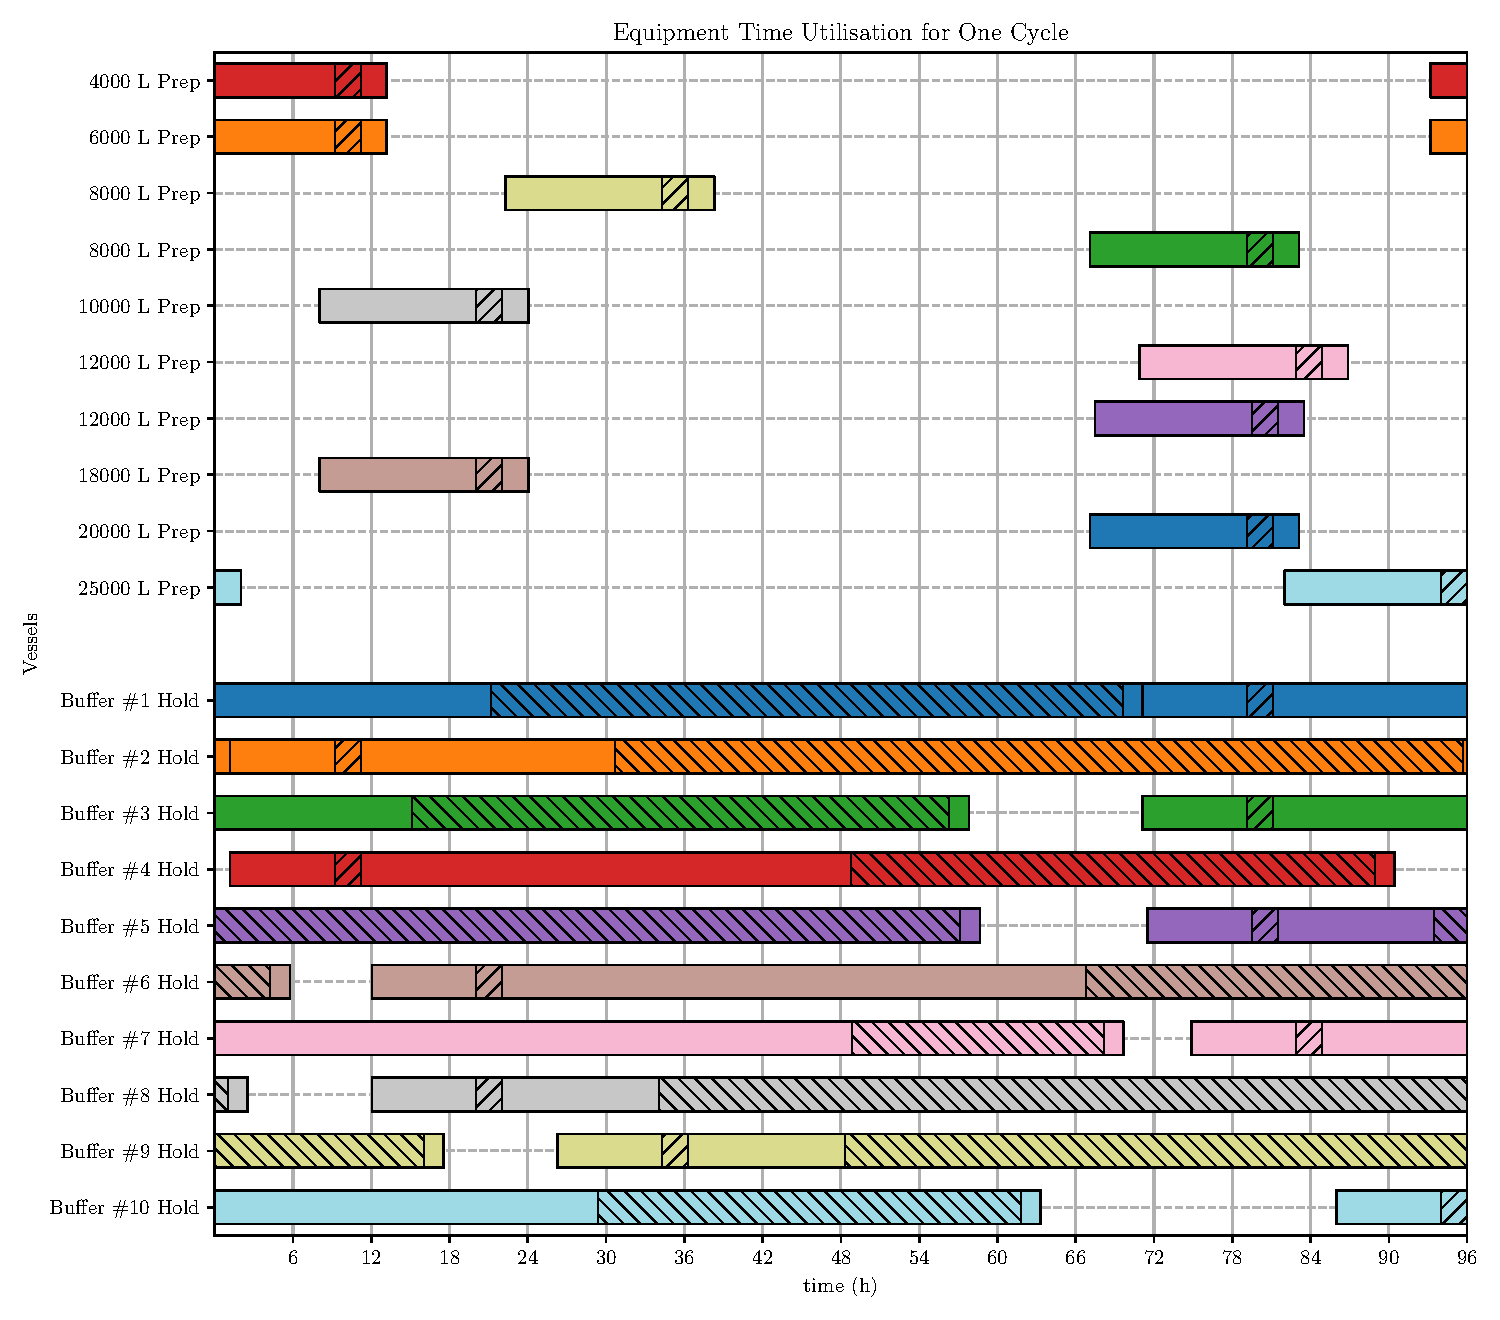
\includegraphics[angle=0,scale=0.8]{./figures/plot1.pdf}
    \caption{Equipment time utilisation for random example}
    \label{fig.etu1}
\end{figure}
Each horizontal dotted line represents a piece of equipment (preparation or
hold vessels in this case).
The presence of a bar on a dotted line indicates that the respective piece of
equipment is in use.  
The hatched bars indicate transfers, with backslash hatching representing the
transfer from the buffer preparation vessel to the buffer hold vessel and
forward-slash hatching representing the transfer of buffer from the hold vessel
to the process.
The latter is shown as a contiguous bar in the hold vessel, representing the
period from the start of the first use to the end of the last use of the buffer
in a given batch, although the demand from the process may be discontinuous.

Note that the time window shown in \hyperref[fig.etu1]{Figure \ref*{fig.etu1}}
displays a single cycle at steady-state; the next cycle and the previous cycle
would be identical.
The offset of the single-cycle window is somewhat arbitrary; the
visible window can be thought of as a cylinder that has been cut at right a
angles to its ends and flattened out.

It should be noted also that \hyperref[fig.etu1]{Figure \ref*{fig.etu1}}
does not highlight the batches to which the procedures belong.
The entire downstream process may take more than one cycle to complete, so the
window visible in the plot could be showing buffer preparation and hold
procedures from several successive batches.

The visual output of an equipment time utilisation plot provides a useful
method for validating results.
As the model detailed in 
\hyperref[C.methodology]{Chapter \ref*{C.methodology}} was being developed,
such plots were a useful way of highlighting logical flaws or bugs in the code.
With the finished model, such plots are a useful tool for convincing
colleagues and clients that a proposed vessel selection is feasible.

\section{Complexity}\label{S.complexity}
The notation for complexity in this section is according to \citet{Knuth:1976}.

The problem complexity depends on both the number of buffers, $\mathcal{N}$,
and the number of vessels, $\mathcal{M}$.
The complexity may be evaluated in terms of both the number of variables and
the number of equations in the problem.
The complexity of the basic and complete problems are summarised in tables
\ref{tbl.complexity1} and \ref{tbl.complexity1b}.
For example, a complete problem with twelve buffers and twelve vessels has
\num{2281} equations in \num{1206} variables.
\begin{table}[t]
    \centering
    \caption{Model complexity -- variables}
    \label{tbl.complexity1}
    \begin{tabular}{l | c }
        model & no. of variables \\ \hline
        basic & $\mathcal{N}^2 + \mathcal{N} \mathcal{M}$\\
        complete & $\mathcal{N} {{\mathcal{N}}\choose{2}} + \mathcal{N}^2
            + {{\mathcal{N}}\choose{2}} + \mathcal{N} \mathcal{M}
            + 5\mathcal{N}$\\
    \end{tabular}
\end{table}
\begin{table}[t]
    \centering
    \caption{Model complexity -- equations}
    \label{tbl.complexity1b}
    \begin{tabular}{l | c }
        model & no. of equations\\ \hline
        basic & $2\mathcal{N}^2 + 3\mathcal{N} + 1$\\
        complete  & $2\mathcal{N}{{\mathcal{N}}\choose{2}} 
            + 4{{\mathcal{N}}\choose{2}} + 2\mathcal{N}^2 + 12\mathcal{N} +1$\\
    \end{tabular}
\end{table}
\begin{table}[t]
    \centering
    \caption{Simplified model complexity}
    \label{tbl.complexity2}
    \begin{tabular}{l | c | c}
        model & no. of variables & no. of equations\\ \hline
        basic & $2\mathcal{N}^2$ & $2\mathcal{N}^2 + 3\mathcal{N} + 1$\\
        complete & $\tfrac{1}{2}\mathcal{N}^{3} + \tfrac{5}{2}\mathcal{N}^{2}
                    + 5\mathcal{N}^{3}$
            & $\mathcal{N}^{3} + 4\mathcal{N}^{2} + 12\mathcal{N} + 1$\\
    \end{tabular}
\end{table}

Noting that there is a weak dependence on $\mathcal{M}$ and that, as the problem
grows larger in terms of $\mathcal{N}$, it is likely that $\mathcal{M}$ will
reach a maximum value, the approximation $\mathcal{M} \approx \mathcal{N}$ may
be used as a conservative simplification when considering complexity (see
\hyperref[tbl.complexity2]{Table \ref*{tbl.complexity2}}).
Plots of the functions in
\hyperref[tbl.complexity2]{Table \ref*{tbl.complexity2}} are given in
Figures \ref{fig.dims} and \ref{fig.eqns}.


For the simple model, we can see that both the number of variables and the
number of equations is $\Theta \left( \mathcal{N}^2 \right)$.

Note that ${{\mathcal{N}}\choose{2}}$ is $\Theta \left( \mathcal{N}^2 \right)$.
Accordingly, for the complete model, the number of variables is 
$\Theta \left( \mathcal{N}^3 \right)$ and the number of equations is
$\Theta \left( \mathcal{N}^2 \right)$.

\begin{figure}
    \centering
    \includegraphics{./figures/variables.pdf}
    \caption{Model complexity -- variables}
    \label{fig.dims}
\end{figure}
\begin{figure}
    \centering
    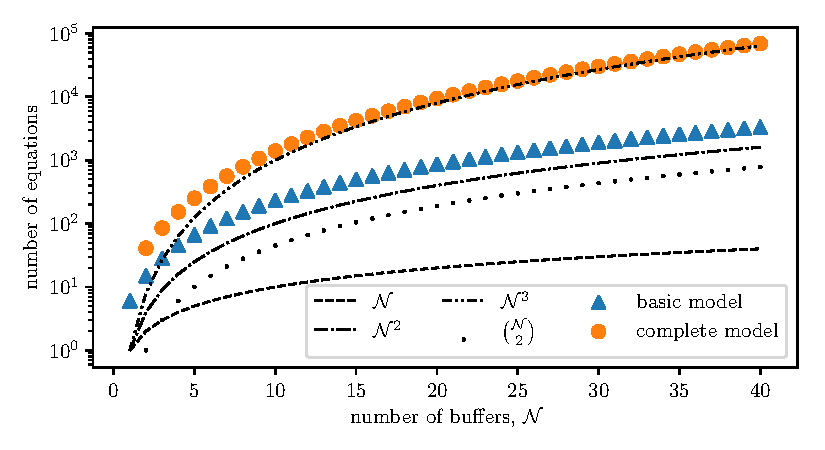
\includegraphics{./figures/equations.pdf}
    \caption{Model complexity -- equations}
    \label{fig.eqns}
\end{figure}

\section{Solution Time}\label{S.soltime}
Using the parameters data set given in 
\hyperref[tbl.parameters]{Table \ref*{tbl.parameters}} and the vessels data set
given in \hyperref[tbl.vessel]{Table \ref*{tbl.vessel}}, the time taken for
the CPLEX solver to reach a feasible solution was evaluated.

The runs were carried out on a computer with 16 GB of RAM and an Intel 3770K
processor (four physical cores; eight virtual cores, running at
 \SIrange{3.5}{3.9}{\GHz}).
The operating system was Arch Linux 64 bit (rolling release).
It was note that the CPLEX solver uses multi-threading effectively, as all eight
virtual cores were running at \SI{100}{\%} fairly consistently during the runs
(the usage tended to dip slightly at the start and end of each run).
RAM usage was not significant, so the 

For a set of problem sizes (i.e. values of $\mathcal{N}$), 100 random data sets
were generated for each problem size and the solution durations were recorded.
A box plot of the durations is shown in 
\hyperref[fig.timing]{Figure \ref*{fig.timing}}.
A total of \num{1000} runs were performed to generate
\hyperref[fig.timing]{Figure \ref*{fig.timing}} and for each run, an optimal
solution was found.
Note that there are several slow outliers for each problem size.
In the case of $\mathcal{N}=20$, the highest outlier is approximately two
orders of magnitude greater than the mean duration, indicating a high degree
of variability.

\textbf{TODO: Other solvers}

\begin{figure}
    \label{fig.timing}
    \centering
    \includegraphics{./figures/timing.pdf}
    \caption{Solution time as a function of buffer count}
\end{figure}

